%-*- mode: LaTeX; -*-
%PL
	%General about excitation and recombination, luminescence 
		%On phonons and replicas
		%On the method of finding stress using phonons
		%On doped materials, and finding their levels using PL
		%On Excitons, binding energies
			%Bound excitons and free excitons
			
	%Describe the method of finding the dopant concentration
			
		
	%Describe the setup
		%Laser and optics
		%Spectrometer
		%RT vs LT

	
\section{Photoluminescence spectroscopy}
\label{sec:pl}
Photoluminescence (PL) spectroscopy is a very powerful tool in optical characterization of semiconductors. It is a non-invasive and fast technique. PL is similar to absorption spectroscopy in that a light source is aimed at the sample to induce electron excitations. As the electrons deexcite (recombine with holes), a photon is emitted. These emitted photons are called the \emph{luminescence} of the sample, and is what is measured in PL spectroscopy. Figure \ref{fig:pl1} shows a schematic of the method of generating luminescence. As the laser beam (A) hits the sample (B), photoluminescence (C) is generated. As not all laser light is absorbed, some of the light reflects away form the sample (D). 

\begin{figure}[h]
\begin{center}
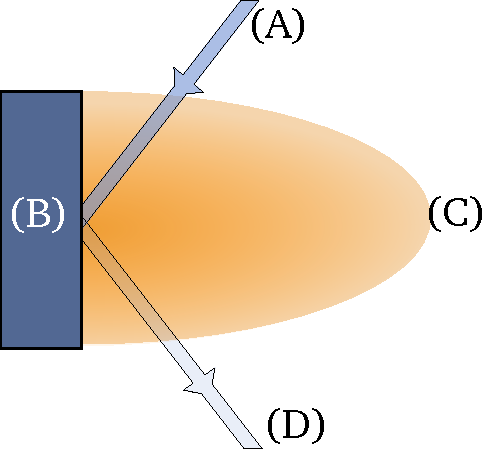
\includegraphics[scale=0.5]{PL1.pdf}
\caption{Photoluminescence induced from a sample by a laser beam. 
\label{fig:pl1}}
\end{center}
\end{figure}

The process of excitation and recombination is shown in figure \ref{fig:pl2}, where a photon is captured (a) and generates an \emph{electron hole pair (EHP)} (b). The EHP then recombines and emits a photon of energy corresponding to the band gap, E$_g$ (c). 

\begin{figure}[h]
\begin{center}
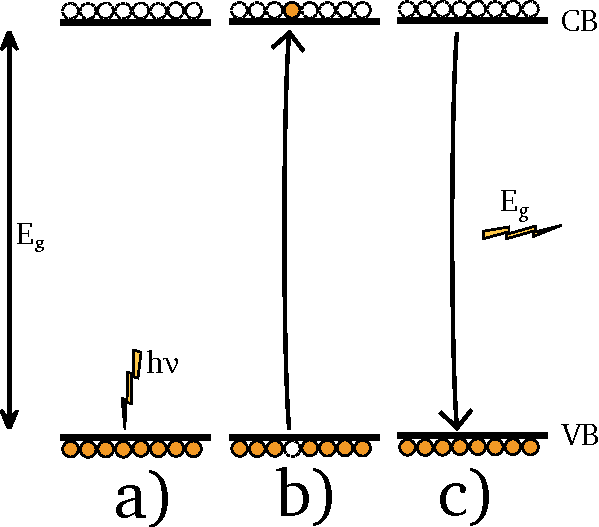
\includegraphics[scale=0.6]{PL2.pdf}
\caption{An EHP is generated by capture of a photon with energy $h\nu$ (a), (b). The EHP recombines to emit a photon of energy E$_g$.
\label{fig:pl2}}
\end{center}
\end{figure}

To generate an EHP by a transition between the valence and conduction bands, the energy of the light must be greater than the band gap. This is in accordance with the principle of conservation of energy. The laser must be chosen accordingly. Not only the energy is conserved in this process, but as is the momentum. Since SiC is an indirect semiconductor (see figure \ref{fig:band}), an electron moving across the band gap has a change in momentum. The light momentum is far too small to compensate for this change. To allow the EHP to be generated, the change in momentum is contributed by phonons. As the transition occurs, a phonon is either created or annihilated. The phonon energies for the different modes in 3C-SiC are described in section \ref{sec:band_structure}. The phonons show in PL spectra as lines with energies slightly smaller than the value of the acctual energy transition, called the \emph{zero phonon line (ZPL)}. The phonon lines are called \emph{phonon replicas}. 

The phonon replica lines can be used to investigate the biaxial stress in the material. The PL intensity of the transverse optical and longitudinal acoustic modes should be the same if the material is without internal stress. Hence the ratio 
\[\frac{I_{\mathrm{LA}}}{I_{\mathrm{TO}}}\]
should be near unity in good quality samples \cite{Sun2012b}. Here I$_\mathrm{LA}$ and I$_\mathrm{TO}$ are PL intensities of arbitrary units. The phonon lines can aslo be used to estimate the doping concentration of a dopant. Camassel et al. have introduced a method where the full width at half maximum (FWHM) value of the TA-line is used for this purpose. 

If doping levels are introduced in the band structure, then transitions can occur between such levels and the bands. In this case there will be another set of ZPL and phonon replicas at the new transition energy. The band structure can thus be inferred from the PL spectrum. 

As the EHP are generated, the electron and hole will interact with each other through the Coulomb force if they are near enough to each other. Due to their charge difference, they will start to orbit each other. This is called the \emph{exciton} quasiparticle. The energy of recombination of an exciton is slightly shifted from a normal recombination of a EHP, due to the potential energy from the Coulomb interaction. At room temperature the thermal energy from the ambient is generally high enough to split the exciton into a free electron and hole, so the excitons are not seen in the PL spectrum. At very low temperatures there is not enough energy to split the exciton, so the PL spectrum shows this shift in the recombination energy attributed to the Coulomb interaction. Some excitons can freely move in the sample, but some excitons bind to impurities in the sample. There is a small energy difference in the free and bound excitons attributed to the binding energy to the impurity. It is thus possible to distinguish from the free and bound excitons in the PL spectrum. They show that the concentration of nitrogen donors in the sample is proportional to the FWHM, $\Gamma$, through the formula
\begin{equation}
\label{eq:fwhm}
\Gamma_\mathrm{TA} = A[N]^{1/n}.
\end{equation}
Here A and n are constants and [N] denotes the concentration on nitrogen donors. This method has however not been validated for acceptor type impurities. 

The PL setup can be described as follows. An optical setup is used to focus a laser beam on a sample. The emitted photoluminescence passes through another optical setup and is focused into a spectrometer. The spectrometer separates the incident light by wavelength, generally by the use of a grating. Photons with a given wavelength can now be collected by a photomultiplier tube or a CCD camera, and the photon intensity for the wavelength spectrum can be computed. Light is captured during a set time (generally ranging between seconds to minutes depending on the sample and setup). 

The sample can be placed in a cryostat to measure the luminescence at low temperature, or measurements can be performed in room temperature. Various types of cryostats exist, generally using either liquid nitrogen or helium. In this work results have been obtained using room temperature measurements and by the use of a liquid helium cryostat. 






































